%\documentclass{sig-alternate-05-2015}
%\documentclass{article}
\documentclass{article}
\usepackage{lipsum}
\usepackage[utf8]{inputenc}
\usepackage{multicol}
\usepackage{listings}
\usepackage{verbatim}
\usepackage{color}
\usepackage{geometry}
\usepackage{float}
\floatstyle{boxed}
\restylefloat{figure}
\usepackage{amsmath}
\usepackage[svgnames]{xcolor}
\definecolor{ocre}{RGB}{243,102,25}
\usepackage{caption}
\usepackage[font={color=black},figurename=Fig.,labelfont={it}]{caption}
%\captionsetup{labelformat=empty,color=red}
\usepackage{pdflscape}
\usepackage{hyperref}
\setlength{\belowcaptionskip}{-10pt}
\setlength{\abovecaptionskip}{-30pt}

\usepackage{graphicx}
\definecolor{codegreen}{rgb}{0,0.6,0}
\definecolor{codegray}{rgb}{0.5,0.5,0.5}
\definecolor{codepurple}{rgb}{0.58,0,0.82}
\definecolor{backcolour}{rgb}{0.95,0.95,0.92}
\geometry{
	a4paper,
	total={180mm,235mm},
	left=19mm,
	right=19mm,
	top=19mm,
	bottom=10mm
}
\lstdefinestyle{mystyle}{
	backgroundcolor=\color{backcolour},   
	commentstyle=\color{codegreen},
	keywordstyle=\color{blue},
	numberstyle=\tiny\color{codegray},
	stringstyle=\color{codepurple},
	basicstyle=\footnotesize,
	breakatwhitespace=false,         
	breaklines=true,                 
	captionpos=b,                    
	keepspaces=true,                 
	numbers=left,                    
	numbersep=5pt,                  
	showspaces=false,                
	showstringspaces=false,
	showtabs=false,                  
	tabsize=2
}

\lstset{style=mystyle}
\usepackage{lipsum}
\usepackage{titlesec}
\titlespacing\section{0pt}{4pt plus 4pt minus 2pt}{0pt plus 2pt minus 2pt}
\titlespacing\subsection{0pt}{12pt plus 4pt minus 2pt}{0pt plus 2pt minus 2pt}
\titlespacing\subsubsection{0pt}{12pt plus 4pt minus 2pt}{0pt plus 2pt minus 2pt}
\begin{document}

% Copyright
\title{Votes Prediction In Stackoverflow Answers\\
Faculty of Science and Technology\\University of Tartu}
\author{
Aqeel Labash\\aqeel.labash@gmail.com\\ \textbf{Supervisor}\\
       Tambet Matiisen}
\maketitle
\setlength\columnsep{15pt} 
\begin{multicols*}{2}
\begin{flushleft}
\section*{abstract}
The aim of this project is to see if we can truly predict number of votes a stackoverflow answer can get. That is depending only on the question and the answer text using LSTM \footnote{Long-Short-Term-Memory} network.
\section*{Keywords}
Deep Learning;Stackoverflow votes prediction;Long Short Term Memory
\section{Introduction}
Every day around 10-20M \footnote{Million} views, 4-10M users visit stackoverflow website \cite{1}. Every minute 4.6 answers,2.84 questions. With 11,573,980 questions and 18,713,658 answers, 5,509,974 users ,56,372,889 comments.\cite{2}This huge amount of data exist on stackoverflow website. Where people can post questions and they are answered by the users. It has a feature which is, each answer can get votes based on the quality of the answer. Consequently, Voting is the vital factor that determine how good is an answer for specific question. Therefore, being able to predict the expected number of votes before even submitting it is the major motivation for this project.
\section{Background}
\subsection{Deep Learning}
There is many definitions for deep learning one of them is:"A class  of machine learning techniques that exploit many layers of non-linear information processing for supervised or unsupervised feature extraction and transformation, and for pattern analysis and classification."\cite{3} another definition explain it as an algorithms based sub-field in machine learning to learn multiple levels in order to model complex relationship between features.\cite{3} One of the methods used in deep learning is Recurrent Neural Networks.
\subsection{Recurrent Neural Networks}
It is a class of artificial neural network. It is renowned for it's dependency on previous information (sequences).\cite{5}\cite{6}Which traditional neural networks lake because it treat all input,output as independent from each other which is not suitable for all cases.\cite{6} Specially when we are working with natural languages where each word depend on series of previous words. 
\begin{figure}[H]
\centering
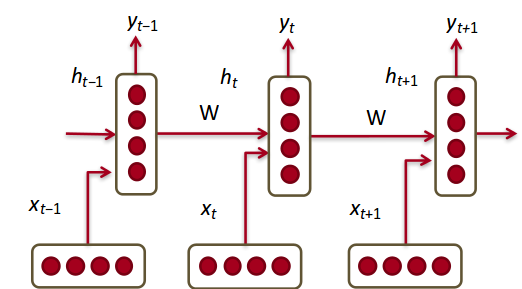
\includegraphics[scale=0.4]{RNN.png}
\caption{Recurrent Nerural Network}
\end{figure}
In figure 1 we can see that the result at certain time \(y_t\) depend on \(x_{t-1},x_t\).But it does not depend on \(x_{t-1}\) directly, weights have to be applied first
\subsection{Long Short Term Memory}
Long Short Term Memory is a Recurrent neural network that introduced memory cell.Memory cell prevent gradient vanishing and explosion by using 4 gates Shown in Fig 2.Those gates modulate environment-memoery cell interaction.
\begin{figure}[H]
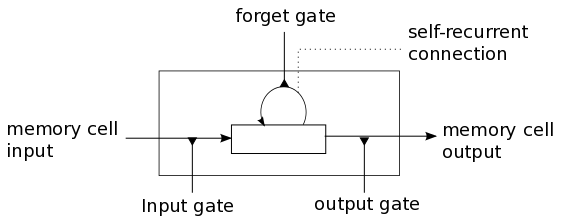
\includegraphics[scale=0.43]{memory_cell.png}
\caption{ Memory cell \cite{8}}
\end{figure}
\begin{figure*}
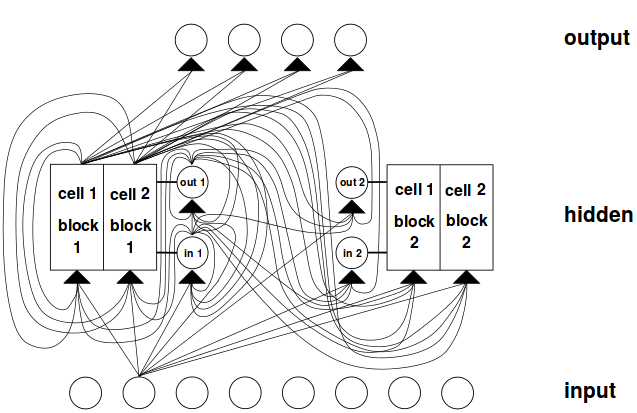
\includegraphics[width=17cm]{lstm.png}
\caption{Example of a net with 2 memory cell blocks of size 2\cite{9}}
\end{figure*}
\textbf{Self-recurrent connection:}it has a weight of 1.It's main task to keep memory cell state constant regardless of any interference.\\
\textbf{Input gate:} allow or prevent incoming signal from changing the memory cell state.\\
\textbf{Output gate:} responsible of allowing the memory cell to affect other neurons.\\
\textbf{Forget gate:} this gate inflect self-recurrent connection to allow or prevent it from remembering the previous state.
\subsection{Fully connected layer}
A fully connected layer is when every neuron from previous layer is connected to every neuron on the next layer.As shown in Figure 4
\begin{figure}[H]
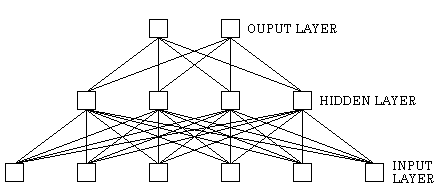
\includegraphics[scale=0.54]{FCN.png}
\caption{Fully connected neural network \cite{10}}
\end{figure}
\section{Dataset}
The data set I used to optimize the parameters were from astronomy.stackexchange.com. It has around 4536 answers and 2738 answered question. I picked this because it is not so large to take long time in processing nor very small.
\subsection{Preprocessing}
Before using the data It should be organized and cleaned to get better result.
\subsubsection{Organize Data}
In this level the task was to get the data that we might use, from XML files to CSV file.
\subsubsection{Remove HTML tags}
When working with data from the web usually it contain html  tags which was the first thing to do. For this I used Regular expression library in python
\subsubsection{Remove Special Characters}
The answers and questions contained new lines and quotes which needed to be removed to generate a valid CSV file.
\subsubsection{Remove Stop Words}
Stop words usually have high frequency which lead for them to act as noise more than features.To achieve this task I used nltk library.
\subsubsection{Stem Words}
Stem words help in decreasing the dictionary size.I used Porter algorithm to stem the words.
\subsection{Simple Statistics}
The following table so some measures for words in questions and answers text.\\
\begin{tabular}{|c|c|c|c|c|}
\hline
&Min&Mean&Max&Median\\ \hline
Q&3&50&3095&38\\ \hline 
A&3&117&2195&86\\ \hline
\end{tabular}\\
\vspace{2mm}
The answers \textbf{average} score : 3.34,\textbf{median}:2.\\
The Questions \textbf{average} score : 4.82,\textbf{median}:3.\\
The total number of unique words : 60644.
\begin{figure}[H]
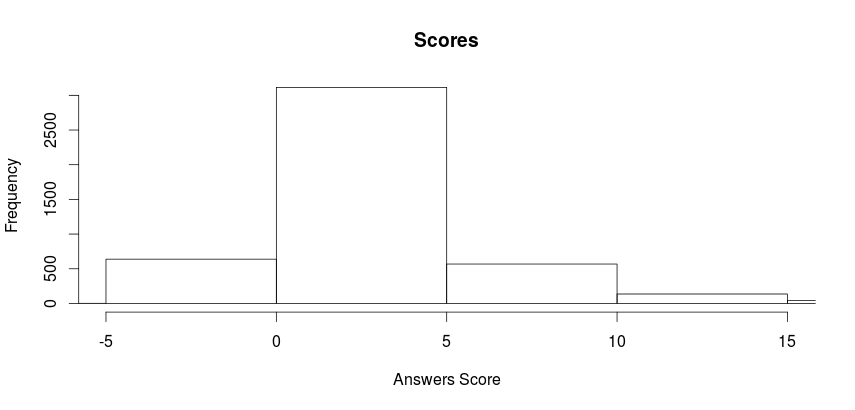
\includegraphics[scale=0.29]{his.png}
\caption{Distribution of answers over scores(Votes)}
\end{figure}
Figure 5 shows the distribution of answers over votes. where we can clearly see that most questions lay between 0-5 votes.
\section{Model}
\subsection{Question Answer Representation}
To represent the data, I used dictionary index so  each word would be weighted as a unique word.Using count,binary representation for the words might loose the uniqueness of the words.\\
For the length of question and answer vectors I used the mean value of length.The increase in vectors length will lead to increase of MSE (Mean Square Error).After that the result from both networks were merged to be fed to full connected layer.
\subsection{LSTM Model}
The questions and answers were fed to two LSTM networks with the same hidden layer size.
\subsubsection{Hidden layer size}
To decide the best hidden layer size many experiments were done to optimize it.I tried the values (5,15,25,100,150), results in figure 6
\begin{figure}[H]
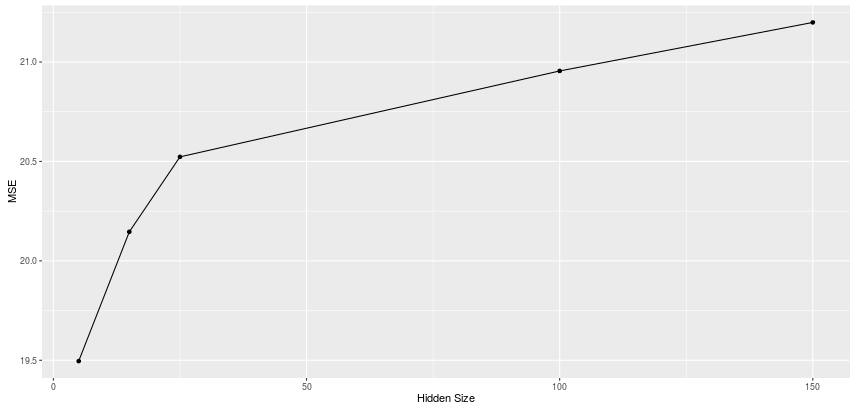
\includegraphics[scale=0.27]{hiddenSize.png}
\caption{Shows test set MSE changes over different hidden layer size}
\end{figure}
From the figure we can see that the best hidden layer size was 5. 
\subsection{Full connected layer}
At the end there is a fully connected layer that take as input the merged vector of questions and answers networks and output a single value that represent the prediction.
\subsection{EPOCH}
To select the best epoch number I tested (2,50,100,125,200) and the test MSE was as the following plot:
\begin{figure}[H]
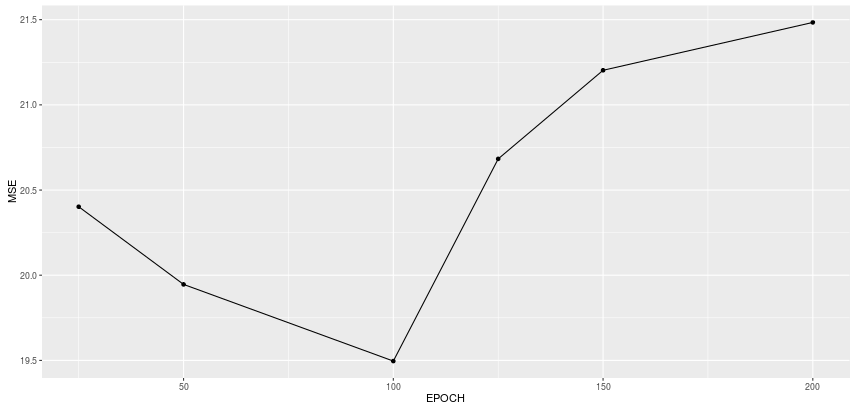
\includegraphics[scale=0.27]{EPOCH.png}
\caption{Shows test set MSE changes over different epoch}
\end{figure}
From figure 7 we can see that the error decreases while going from 25 to 100 and after that is start increasing.
\section{Results}
After finalizing the parameters the lowest MSE achieved was 20.27 for testing and 2.15 for training.Here is some examples:\\
\textbf{Link:}\href{http://astronomy.stackexchange.com/questions/322}{Dark Matter Particle Candidates}\\
\textbf{Score:}6\\
\textbf{Predicted Score:6.19}\\
\textbf{Link:}\href{http://astronomy.stackexchange.com/questions/13301}{Is it odd that our Sun has so many planets?}\\
\textbf{Score:}15\\
\textbf{Predicted Score:11.20}\\
The previous examples score was close some how.\\
To save the space I'll just mention the links.
The following example is the worst prediction in test set :\\
\textbf{Link:}\href{http://astronomy.stackexchange.com/questions/140}{Does the Sun rotate?}
\textbf{Score:}62\\
\textbf{Predicted score:}5.20\\
\textbf{Link:}\href{http://astronomy.stackexchange.com/questions/13559}{How probably is it that galaxies will extinguish?}
\textbf{Score:}-2\\
\textbf{Predicted score:}3.33\\
\textbf{Link:}\href{http://astronomy.stackexchange.com/questions/12385}{Is extraterrestrial mining more difficult or impractical for bodies without plate tectonics?}
\textbf{Score:}0\\
\textbf{Predicted score:}-1.21\\

\section{Discussion}
The final result achieved was  20.27 MSE for testing and 2.15 MSE for training which indicate a clear over fitting. I believe this problem is due to the amount of data used.I'll try to use larger amount of data (as much the server can handle) to inspect the parameters more.But regardless of that point if we take a look at the histogram of prediction and test  (figure 8 \& 9) we can see that the problem happens with the outliers.
\begin{figure}[H]
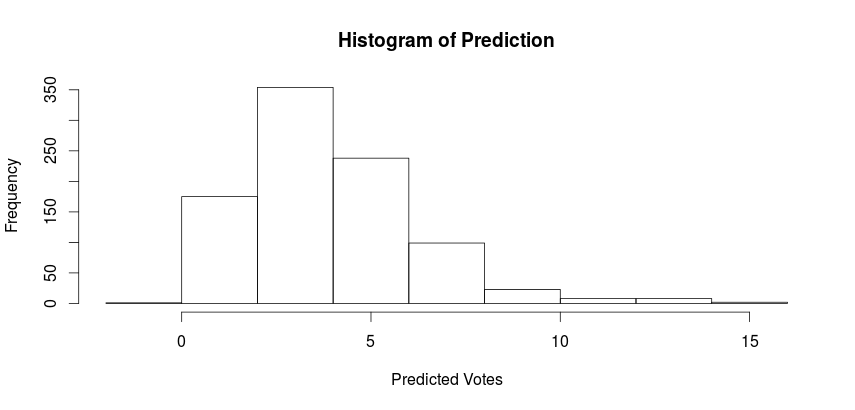
\includegraphics[scale=0.3]{histpredict.png}
\caption{Histogram of votes predicted}
\end{figure}
\begin{figure}[H]
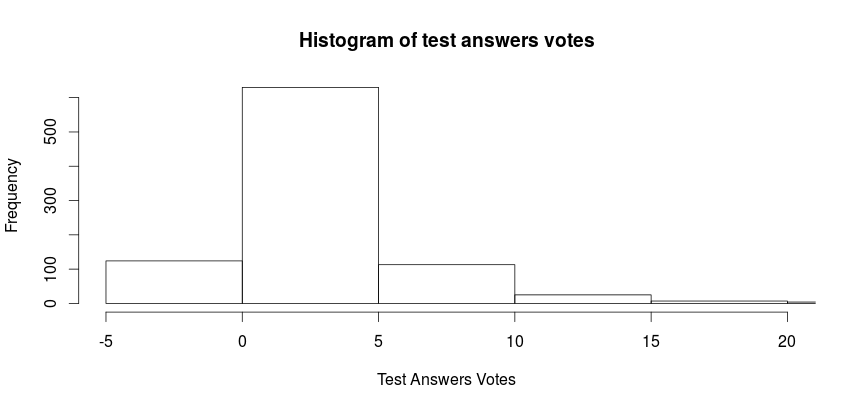
\includegraphics[scale=0.3]{histtest.png}
\caption{Histogram of test set answers votes}
\end{figure}
The following figure shows the density of predicted votes and actual votes in testing set.
\begin{figure}[H]
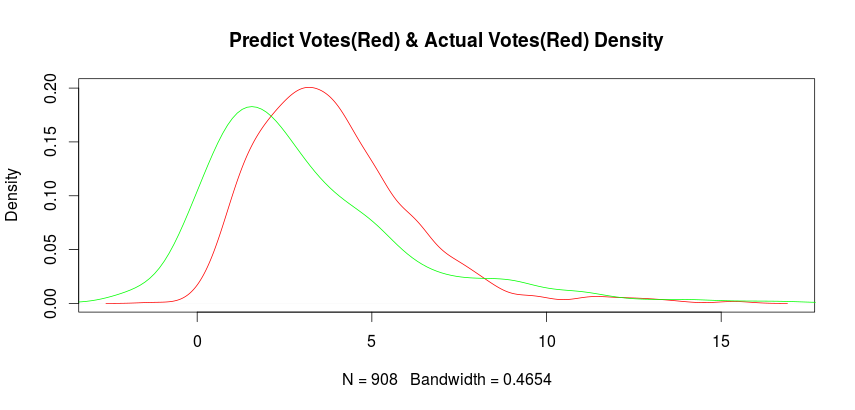
\includegraphics[scale=0.29]{density.png}
\caption{Density of predicted votes vs actual votes}
\end{figure}
\section{Future work}
Firstly, more cleaning for the data would improve the results. I was focused on generating a valid CSV and keep latex code. Which distracted me at some point to do more special characters cleaning.\\
Secondly, I think there is many feature that would decrease the error like:
\begin{enumerate}
\item Question view count: Which represent how much popular the topic is. some times the answer is quite good but it's not popular topic which lead to small amount of votes.
\item Percentage between question view count and question score: This feature would give how good the question is.
\item Date : the older the post is the more chance it has to have more votes.
\item User reputation: reputation of the user who answered question have influence as well on the votes.Users with high reputation usually provide good answers. 
\item User badges: each badge has specific meaning which also can help in determining the quality of the user answers.
\end{enumerate}
Use larger data set and try different Stackoverflow forums would help optimizing the model even more.But it'll need more resources as well.
\section{Conclusion}
In this project Stackoverflow answers votes were used to train a LSTM network to predict the votes.Depending on the current findings the votes could be predicted with acceptable margins considering that only the text were used. Popular topics won't be predicted correctly. The results could be improved by using more samples or including more features related to topics popularity.\\
\textbf{Note:}All code,.tex, .py,.ipython etc.. files available on \href{https://github.com/aqeel13932/RSDM2016/}{Github}
	\begin{thebibliography}{9}
		\bibitem{1}
		https://api.stackexchange.com/docs/info
		\bibitem{2}
		https://www.quantcast.com/stackoverflow.com
		\bibitem{3}
		Deng, L.; Yu, D. (2014). "Deep Learning: Methods and Applications"
		\bibitem{5}
		A. Graves, M. Liwicki, S. Fernandez, R. Bertolami, H. Bunke, J. Schmidhuber. A Novel Connectionist System for Improved Unconstrained Handwriting Recognition. IEEE Transactions on Pattern Analysis and Machine Intelligence, vol. 31, no. 5, 2009.
		\bibitem{6}
		The Unreasonable Effectiveness of Recurrent Neural Networks,	    karpathy.github.io,May 21st, 2015
		\bibitem{7}
		Recurrent Neural Networks Tutorial, Part 1 Introduction to RNNs, Denny Britz, September 17, 2015	
		\bibitem{8}
		http://deeplearning.net/tutorial/lstm.html
		\bibitem{9}
		 Sepp Hochreiter and Jürgen Schmidhuber (1997). "Long short-term memory". Neural Computation 9 (8): 1735–1780.
		 \bibitem{10}
		 Mary Jo Creaney-Stockton,1996, Isolated Word Recognition Using Reduced Connectivity Neural Networks With Non-Linear Time Alignment Methods.
		 
	\end{thebibliography}
\end{flushleft}
\end{multicols*}
\end{document}
